\documentclass[tikz,border=10pt]{standalone}
% No extra libraries needed for this figure.
\begin{document}
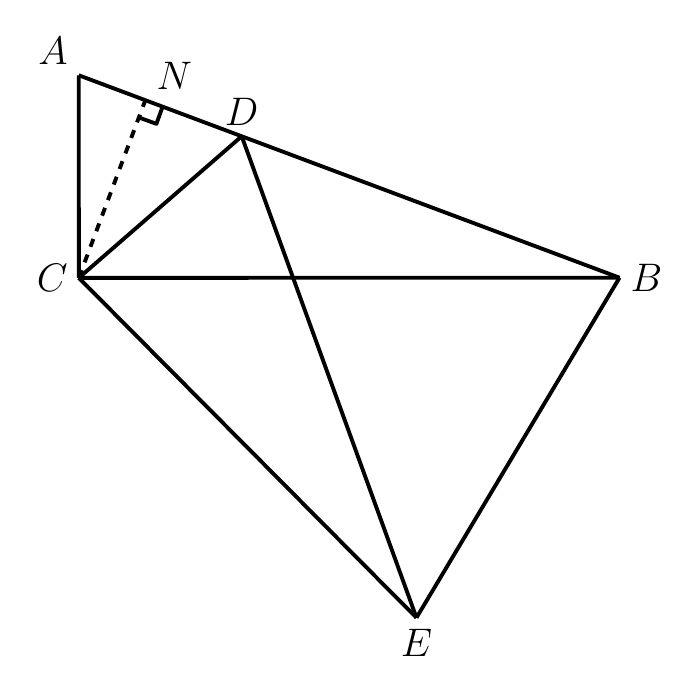
\begin{tikzpicture}[line join=round, line width=1.4pt]
  % Coordinates: scale s = 0.018223 cm/px, centred on ink bbox (cx=245, cy=225), y flipped
  \coordinate (A) at (-3.478545443687297,3.478919254618713);
  \coordinate (N) at (-2.6332057937252253,3.1624652449316133);
  \coordinate (D) at (-1.4090844657705222,2.7042138159442897);
  \coordinate (B) at (3.3886650986241498,0.9081699568926626);
  \coordinate (C) at (-3.477824514165793,0.9062457892368866);
  \coordinate (E) at (0.8099951187246881,-3.410014061624164);

  % Main solid segments
  \draw (A) -- (B);   % line AB (contains D and N)
  \draw (A) -- (C);   % vertical AC
  \draw (C) -- (B);   % horizontal CB
  \draw (C) -- (E);
  \draw (D) -- (E);
  \draw (B) -- (E);
  \draw (C) -- (D);

  % Dashed altitude CN
  \draw[dashed] (C) -- (N);

  % Right-angle mark at N (from mark_points_px converted to cm)
  \draw (-2.413230633315085,3.0824173178794254) -- (-2.4925731346475812,2.8621693445376013) -- (-2.7125482950577218,2.9422172715897887);

  % Labels
  \node[above left] at (A) {\fontsize{14.5}{17.4}\selectfont $A$};
  \node[above right] at (N) {\fontsize{14.5}{17.4}\selectfont $N$};
  \node[above] at (D) {\fontsize{14.5}{17.4}\selectfont $D$};
  \node[right] at (B) {\fontsize{14.5}{17.4}\selectfont $B$};
  \node[left] at (C) {\fontsize{14.5}{17.4}\selectfont $C$};
  \node[below] at (E) {\fontsize{14.5}{17.4}\selectfont $E$};
\end{tikzpicture}
\end{document}
% GEOAGENT_REPAIR_V1 c18a466396f54661 2bc97d7ef165d623ef0e45345a49b24a571f039a6aec851705f14d95f48978a7
